%10MB

\documentclass[10pt,finnish,a5paper,headings=small,twoside=semi]{scrartcl}

\usepackage{fontspec}
\usepackage{babel}
\usepackage{microtype}
\usepackage{multicol}
\usepackage{xcolor}
\usepackage{enumitem}
%\usepackage{ragged2e}
\usepackage{graphicx}
\usepackage{wallpaper}
\usepackage{lipsum}
\usepackage{tcolorbox}
\usepackage[labelformat=empty]{caption}
\usepackage[export]{adjustbox}
\usepackage{calc}

\definecolor{link}{HTML}{05A8F7}

\usepackage[colorlinks,linkcolor=black,urlcolor=link]{hyperref}

\RedeclareSectionCommands[tocraggedentrytext]{section}

%\setlength{\RaggedRightParindent}{\parindent}
%\RaggedRight
\setmainfont[Ligatures=TeX]{Arimo}
\urlstyle{same}
\definecolor{kuru}{HTML}{f7941e}
\setcounter{secnumdepth}{0}
\setcounter{tocdepth}{1}
\addto\captionsfinnish{\renewcommand{\contentsname}{Tässä numerossa:}}
\addtokomafont{sectionentry}{\normalfont}
\addtokomafont{disposition}{\rmfamily}
\addtokomafont{caption}{\footnotesize}
\setkomafont{subsection}{\normalfont\itshape}
\setenumerate{leftmargin=*}
\setitemize{leftmargin=*}
\frenchspacing
\def\UrlBreaks{\do\/\do-}

\begin{document}
\thispagestyle{empty}

\ThisCenterWallPaper{1.10}{kansikuva}

\vspace*{5.70cm}

{\noindent\color{kuru}\begin{tabular}{@{}c@{}}

\includegraphics[width=6cm]{logo} \\
\\
{\large\bfseries 1/2024 Kurkisuon Rusakot ry}
\end{tabular}\par}

\clearpage

\ThisULCornerWallPaper{1}{sisäkansikuva.jpg}

\noindent \textbf{Tassu 1/2024} \\
\noindent ISSN 0783-1536

\vfill

\begin{multicols}{2}
\noindent\textbf{Toimitus:}

Tanguy Gérôme

\href{mailto:tanguy.gerome@gmail.com}{tanguy.gerome@gmail.com}

\medskip

\noindent\textbf{Julkaisija:}

Kurkisuon Rusakot ry, Helsinki

\medskip

\noindent Tarkista lippukunnan ajankohtaiset yhteystiedot nettisivuilta:

\href{https://kurkisuonrusakot.wordpress.com/}{kurkisuonrusakot.wordpress.com}

\medskip

\noindent Etu-, sisä- ja takakannen kuvat:

Tanguy Gérôme

\columnbreak

\tableofcontents
\end{multicols}

\clearpage\section{Lippukunnanjohtajan tervehdys}

%\medskip

%\begin{multicols}{2}

%\columnbreak

\noindent äääää äääää äääää äääää äääää äääää äääää äääää äääää äääää äääää äääää äääää äääää äääää äääää äääää äääää äääää äääää äääää äääää äääää äääää äääää äääää äääää äääääääääääääääääääääääääääääääää ääääää

öööööööö öööööööö öööööööö öööööööö öööööööö öööööööö öööööööö öööööööö öööööööö öööööööö öööööööö öööööööö öööööööö öööööööö öööööööö öööööööö öööööööö öööööööö öööööööö öööööööö öööööööö öööööööö öööööööö öööööööö öööööööö öööööööö öööööööö! \\

\noindent LPKJ Janne

\medskip
\noindent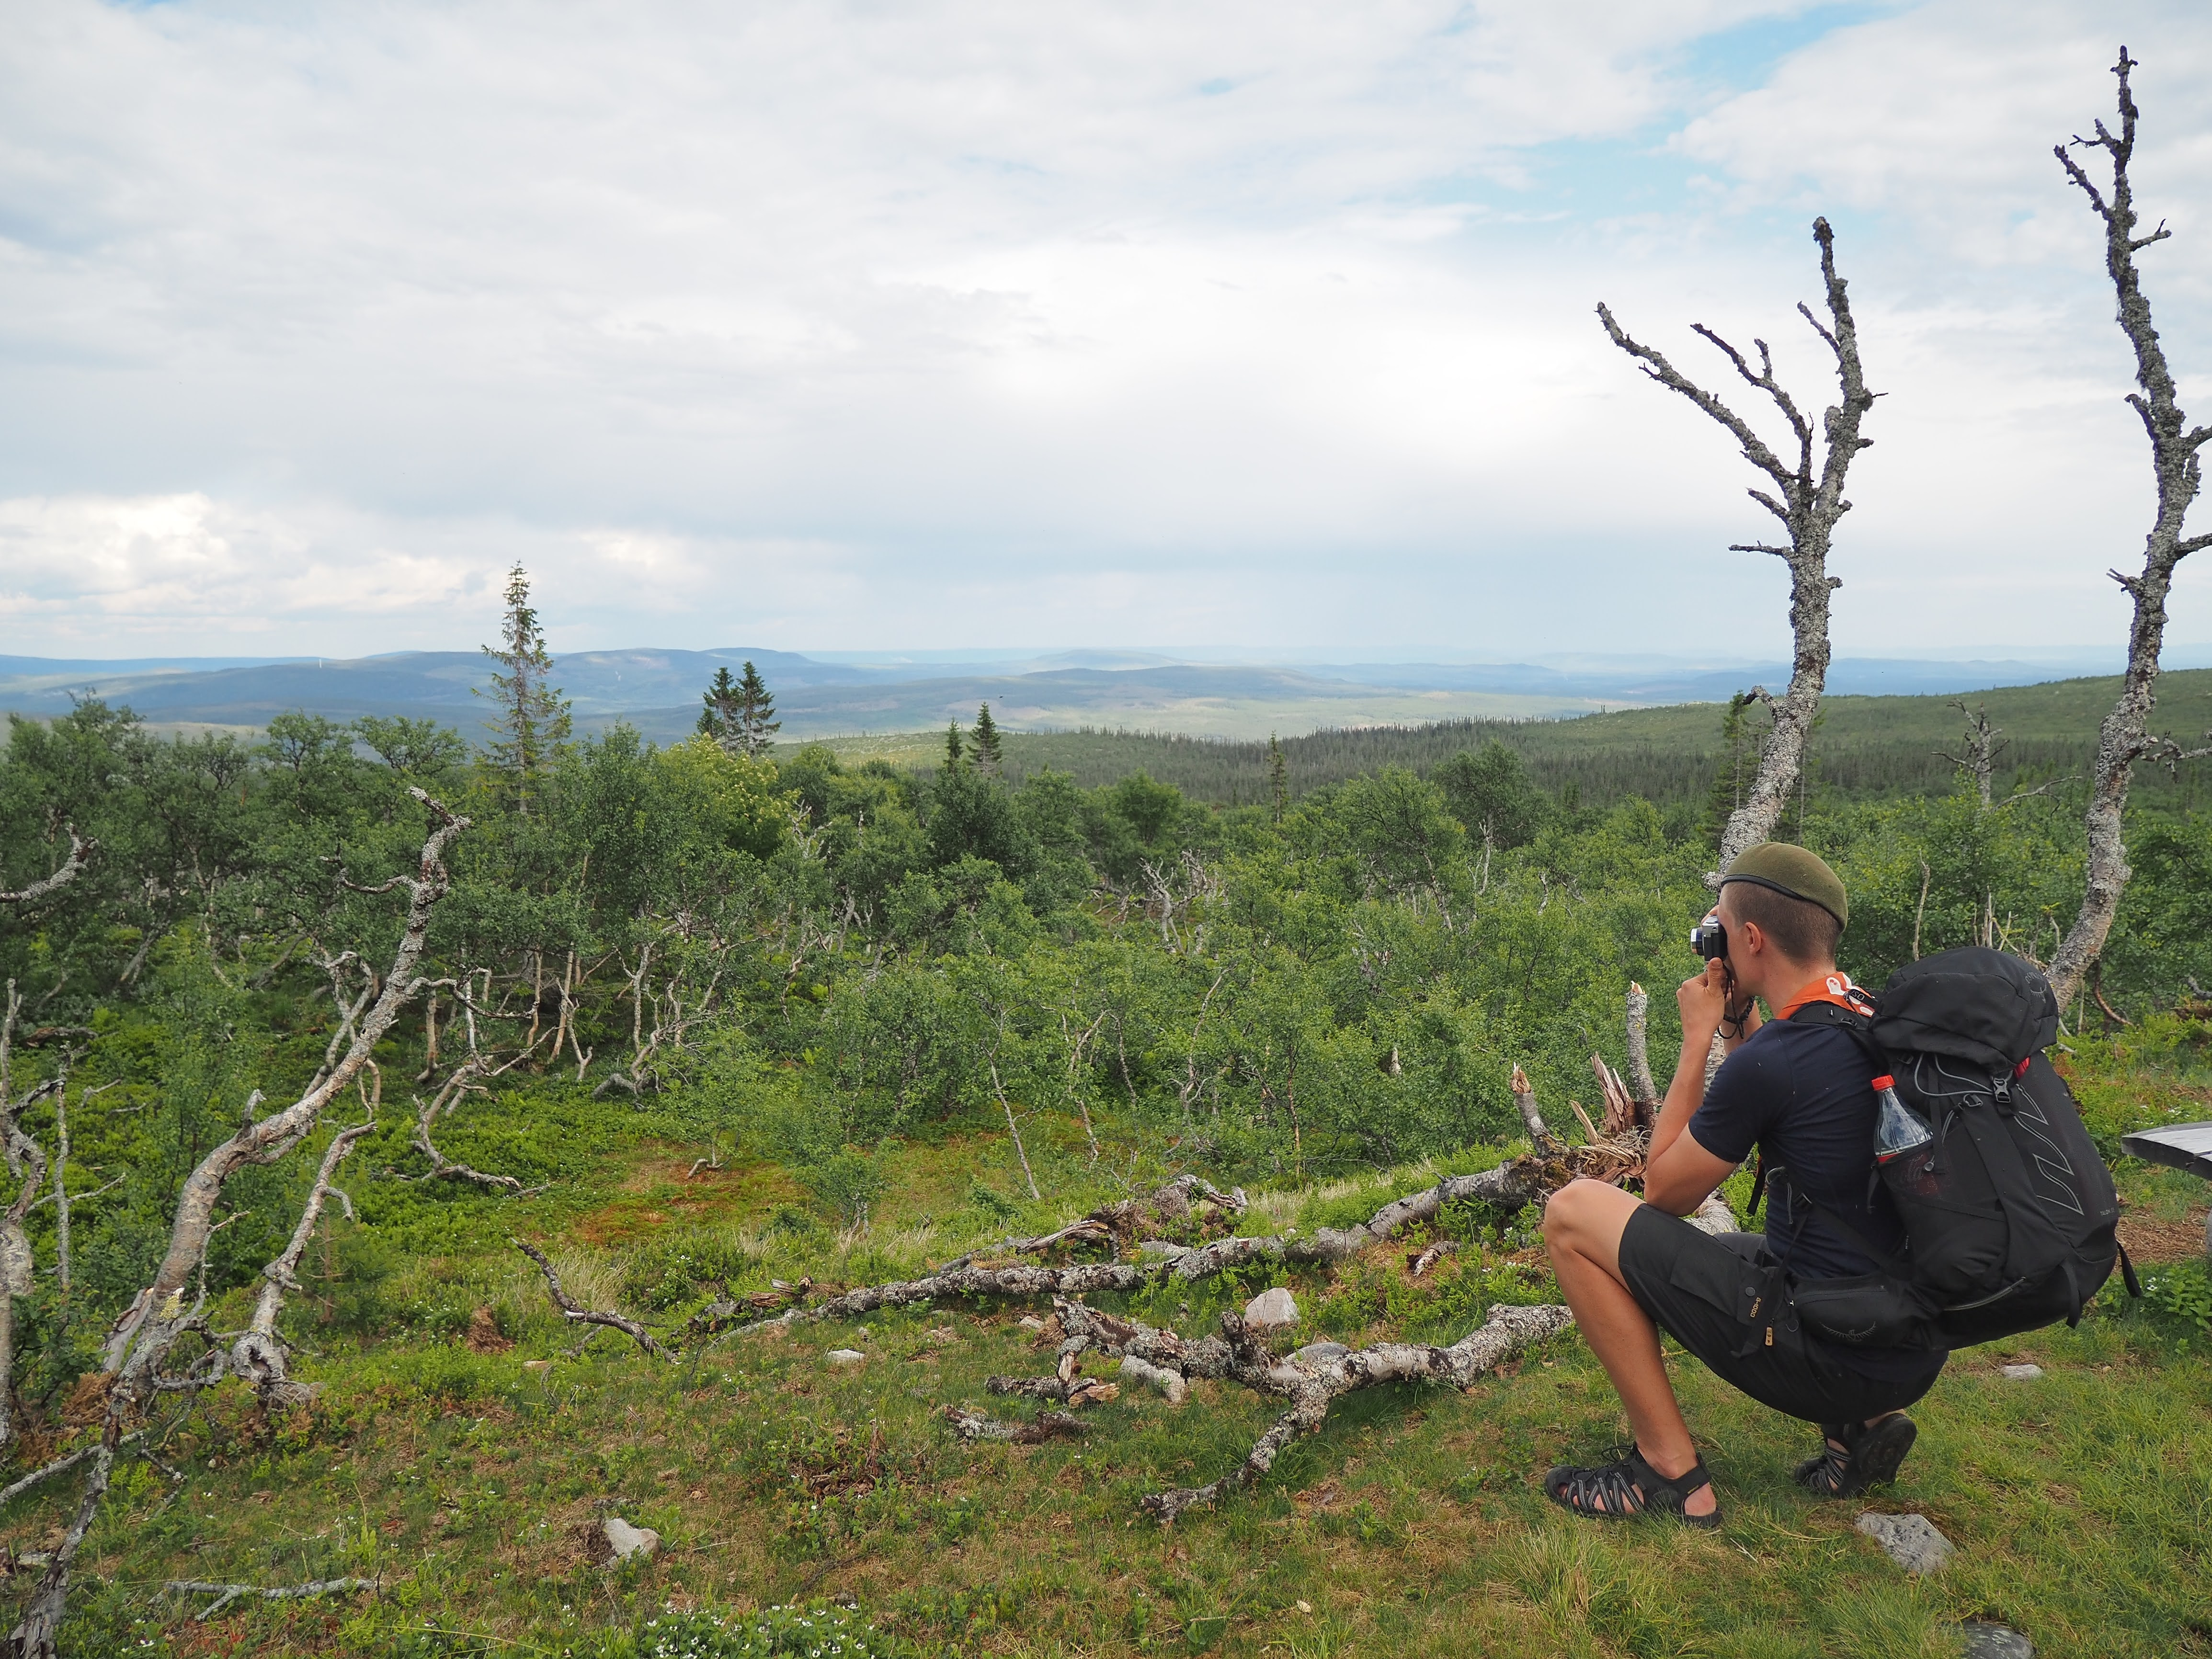
\includegraphics[width=\linewidth]{lpkjtervehdys}

\medskip
\noindent Kuva Tanguy Gérôme

%\end{multicols}

%\clearpage\section{Lippukunnan kevät 2020: retkiä ja etäpartiota}
%
%Vuoden alussa kukaan tuskin arvasi miten poikkeuksellinen partiokeväästä 2020 tulisi. Tassun kuvareportaasin myötä pääsemme kaikki palaamaan alkukevään retkiin ja poikkeusolojen aikaiseen toimintaan.
%
%\vspace*{-.25cm}
%
%\subsection{Tarpojaosaston retki 28.2.–1.3. @ Mörrimöykky} 
%
%\begin{figure}[!h]
%\centering
%\begin{minipage}[t]{.5\linewidth-.5\columnsep}
%\includegraphics[width=\linewidth]{IMG-20200229-WA0004}
%\caption{Yhden rusakon syntymäpäivää vietettiin Mörrimöykyn hämärässä tuvassa retkiperjantaina. Retkellä oli tuttujen oranssihuivien lisäksi mukana sinihuivisia Kontutyttöjä, joiden toimesta valmistui myös kakkutarjoilu.}
%\end{minipage} \hfill \begin{minipage}[t]{.5\linewidth-.5\columnsep}
%\includegraphics[width=\linewidth]{2256153000103720180}
%\caption{Tarpojat pääsivät kokeilemaan perinteisiä partiotaitojaan kisan muodossa. Kuvassa \textit{Vitoset}"-vartio näyttää mallia sytykkeiden teossa.}
%\end{minipage}
%
%\vspace*{\columnsep}
%
%\includegraphics[width=\linewidth,clip,trim={0 .5cm 0 .5cm}]{DSC_0062}
%\caption{Voittajaksi selviytyivät \textit{Mörököllit}, jotka tässä kokeilemassa loukkaantuneen siirtämistä ensiapurastilla. Myös nyrjähtäneen nilkan ja silmävamman ensiapua pohdittiin.}
%\end{figure}
%
%\clearpage\subsection{Kolkkaosaston retki 6.–8.3. @ Östersundom}
%
%\begin{figure}[!h]
%\centering
%\begin{minipage}[t]{.5\linewidth-.5\columnsep}
%\includegraphics[width=\linewidth]{2259034453305001497}
%\caption{Kolkat ja Kontutyttöjen sudenpennut matkasivat Östersundomin leirikeskukseen julkisilla kulkuvälineillä.}
%\end{minipage} \hfill \begin{minipage}[t]{.5\linewidth-.5\columnsep}
%\includegraphics[width=\linewidth]{IMG_20200306_183406}
%\caption{Pihamaalle pystytettiin talviteltta, jossa kaikki kolkat pääsivät viettämään toisen yön.}
%\end{minipage}
%
%\vspace*{\columnsep}
%
%\begin{minipage}[t]{.5\linewidth-.5\columnsep}
%\includegraphics[width=\linewidth]{DSC_0067}
%\end{minipage} \hfill \begin{minipage}[t]{.5\linewidth-.5\columnsep}
%\includegraphics[width=\linewidth]{IMG_20200307_134907}
%\end{minipage}
%
%\vspace*{\columnsep}
%
%\includegraphics[width=\linewidth,clip,trim={0 .3cm 0 .8cm}]{2259493996753497985}
%\caption{Lauantaina ohjelmassa oli niin aamujumppa, huispausta kuin telttasaunan rakentamista. Myöhemmin päästiin nauttimaan myös mainioista löylyistä!}
%\end{figure}
%
%\clearpage
%
%\ThisULCornerWallPaper{1}{2259730771254105316}
%
%~\vspace*{7.7cm}
%
%\begin{figure}[!h]
%\centering
%\caption{Illalla kokoonnuttiin nuotiolle kertomaan vitsejä, laulamaan lauluja ja paistamaan lettuja.}
%
%\vspace*{\columnsep}
%
%\includegraphics[width=\linewidth,clip,trim={0 .3cm 0 0}]{2260220549787494712}
%\caption{Sunnuntaina kolkat valmistivat vielä itse lounaaksi herkullista broileririsottoa. Ruoka valmistui mallikkaasti ja suurimmat haasteet kohdattiin trangian tiskaamisessa: risottoriisi kun tarttuu pohjaan palaessaan ikävästi kiinni kattilan pohjaan\ldots}
%\end{figure}
%
%\clearpage\subsection{Kolkkien etäpartiokokoukset}
%
%Lippukunnan molemmat kolkkaparvet kunnostautuivat poikkeusoloista huolimatta aktiivisuudellaan kevään aikana. Videoyhteyden avulla ja pienellä omatoimisuudella nuorimmat rusakot ehtivät puuhailla mm. Muumit ja Itämeri "=aiheisen \#Meidänmeri"-merkin sekä luovaa ajattelua ja ongelmanratkaisua testaavien tehtävien parissa.
%
%\vfill
%
%\begin{figure}[!h]
%\centering
%\begin{minipage}[t]{.5\linewidth-.5\columnsep}
%\includegraphics[width=\linewidth]{2282166614937710220}
%\end{minipage} \hfill \begin{minipage}[t]{.5\linewidth-.5\columnsep}
%\includegraphics[width=\linewidth]{2312603851655313744}
%\end{minipage}
%
%\vspace*{\columnsep}
%
%\begin{minipage}[t]{.5\linewidth-.5\columnsep}
%\includegraphics[width=\linewidth]{2312603851630204015}
%\end{minipage} \hfill \begin{minipage}[t]{.5\linewidth-.5\columnsep}
%\includegraphics[width=\linewidth]{2312603851655317178}
%\end{minipage}
%\end{figure}
%
%\vfill
%
%\noindent Kuvareportaasien kuvat Nonna Kervinen, Mikko Niinimäki, Janne Suomalainen ja Annina Toivakka
%
%\clearpage\section{Kisailua etäyhteydellä – EtäPupu2020}
%
%\begin{figure}[!h]
%\centering
%\includegraphics[width=\linewidth]{2311148361922581157}
%\caption{Kisan aikana sai käyttää luovuuttaan, mm. partioaiheisella luontotaiteella.}
%\end{figure}
%
%\begin{figure}[t]
%\centering
%\begin{minipage}[t]{.333\linewidth-.5\columnsep}
%\includegraphics[width=\linewidth]{97132957_165548654932063_1649771865181908506_n}
%\end{minipage} \hfill \begin{minipage}[t]{.333\linewidth-.5\columnsep}
%\includegraphics[width=\linewidth]{annina.jpg}
%\end{minipage} \hfill \begin{minipage}[t]{.333\linewidth-.5\columnsep}
%\includegraphics[width=\linewidth]{lilja.jpg}
%\end{minipage}
%\caption{Kisaajat tapasivat toisiaan vain videoyhteyden välityksellä, myös tehtävien palautus tapahtui kuvien ja videoiden muodossa.}
%\end{figure}
%
%\begin{multicols}{2}
%\noindent\includegraphics[width=\linewidth,clip,trim={0 .5cm 0 0}]{2311148361947784797}\captionof{figure}[]{Näinkin herkullinen banaanipannukakku valmistui yhdeltä kisaajalta!}
%
%\columnbreak
%
%\noindent Teksti Väinö Syrjälä \\ Kuvat EtäPupun kilpailijat
%
%\medskip
%
%KuRu:n perinteinen, leikkimielinen partiokisa Pupu herätettiin henkiin näin poikkeuskeväänä, tosin vähän erilaisessa muodossa. Vaikka kilpailijoita olikin lopulta mukana vain kolme, saatiin aikaan mukava viikonloppu haastavien tehtävien parissa ja voittajakin löydettiin!
%
%\hspace*{\parindent} Kisan aluksi kokoonnuttiin videoyhteydellä: lähtötehtävänä taiteltiin rusakko"-origamit. Lisäksi päästiin pienelle vierailulle Tukholmaan videon mudossa. Myös lauantai"-illan yhteisen visailun merkeissä ja kisan maalissa sunnuntaina tavattiin etänä. Muutoin rastivihjeitä ja "=tehtäviä ratkottiin omatoimisesti. Nykytekniikka osoitti tässä hyödyllisyytensä, kun kisan etenemistä päästiin “kisakeskuksessa” seuraamaan kisaajien lähettämien kuvien muodossa!
%
%\hspace*{\parindent} Vaikka rastit suoritettinkin kotosalla, pisteitä kerättiin hyvin samantyyppisistä tehtävistä kuin aikaisemmissa Pupu"-kisoissa. Osallistujat pääsivät ratkomaan salakieliä, loihtimaan jälkiruokaherkkuja keittiössä, rakentamaan majaa, vierailemaan virtuaalisessa Suomenlinnassa ja auttamaan äitiä kotitöissä. Välillä myös ulkoiltiin, niin luontotaidetta loihtimassa kuin haastavaa aukkotekstiä sekä kuvasuunnistusta lähimaastossa ratkoen. Tarjoutuipa illalla vielä mahdollisuus bonuspisteisiin auringonlasku valokuvaamalla.
%
%\columnbreak
%
%\noindent\includegraphics[width=\linewidth]{fb635169-3500-444a-b576-57450430f47b}
%
%\medskip
%
%\noindent\includegraphics[width=\linewidth]{51832ba5-58a0-4072-8c16-e8fe962197a3}\captionof{figure}[]{Äidin pikku apulaiselle oli luvassa hyvät pisteet siististä suorituksesta.}
%\end{multicols}
%
%\begin{multicols}{2}
%Lopulta saatiin laskea tarkasti kaikkien tehtävien pisteet; voittajaksi tasaisessa kisassa selvisi Nonna! Kaikille kisaajille on vielä luvassa palkinnot osallistumisesta sopivassa yhteydessä.
%
%\columnbreak
%
%\noindent\includegraphics[width=\linewidth]{cbf913db-8cab-4518-91d0-6f3674b9fd71}\captionof{figure}[]{Aurinko laskee ensimmäisen kisapäivän iltana, kameraa käyttämällä siitäkin irtosi bonuspisteitä tiukkaan taistoon.}
%\end{multicols}
%
%\vfill
%
%\begin{tcolorbox}
%\noindent Kuinka monta kisan rastitehtävän salakielistä sinä olisit ratkaissut? Nyt pääset sinäkin haastamaan päättelykykyäsi – ratkaisut julkaistaan lippukunnan somessa heinäkuun alussa! \begin{enumerate}
%\item nelletsirääv atuus ivus ivelut neukkiek akoj ättävek aattiokrat okuot nuukokuot
%\item hii ni ya kufurahisha sana
%\item becnxäå dnxnxlölylccl äå årywl fnbfncdn
%\item \textcolor{red}{♦A♥6} / \textcolor{red}{♥8}♣Q\textcolor{red}{♥A♥4} / ♠J♣7 / \textcolor{red}{♥8}♠6 / \textcolor{red}{♥3♥J♥Q}♠K / \textcolor{red}{♦3} / \textcolor{red}{♦10♥5} / \textcolor{red}{♥J♦J♦10}♣3 / \textcolor{red}{♦Q♥2}
%\item 112 + 111 + 109 + 112 + 112 + 105 + 118 + 097 + 116 + 112 + 117 + 112 + 117 + 116
%
%= 107 + 110 + 117 + 098 + 098 + 105 + 103 + 107 + 097 + 110 + 105 + 110
%
%= 099 + 104 + 117 + 098 + 098 + 121 + 098 + 117 + 110 + 110 + 121
%\end{enumerate}
%\end{tcolorbox}
%
%\vfill
%
%\noindent Herättikö raportti innostusta kisailuun? \textbf{EtäPupu2.0} tulee vielä kesällä! Ks. lisää sivulta \pageref{tulossa} ja seuraa tiedotusta sähköpostilla.
%
%\clearpage\section{Partiopuuhailua kesälomalle}
%
%Vaikka kesäleirille ei tänä vuonna päästäkkään, voi kesällä puuhailla partiohenkisesti vaikka oman perheen kanssa. Tässä Tassun parhaita vinkkejä!
%
%\begin{multicols}{2}[\subsection{Vinkkejä partiopuuhailuun kotosalla, pihalla tai lähimaastossa}]
%\includegraphics[width=\linewidth]{_7251867}
%
%\columnbreak
%
%\begin{itemize}
%\item Tee päivän hyvä työ ja kerää roskia lähimetsästä.
%\item Tarkkaile luontoa: bongaa lintuja tai hyönteisiä, seuraa kasvien kasvua kesän mittaan.
%\item Istuta kasvi, kukkia tai yrttejä omalle pihalle tai vaikkapa keittiön ikkunalaudalle.
%\item Opettele tai kertaa partiotaitoja: solmuja, karttamerkkejä tai vaikka morseaakkoset – netistä löydät runsaasti hyviä ohjeita.
%\item Tee eväsretki oman perheen kanssa – kauas ei tarvitse lähteä, vaikka vain parvekkeelle tai lähipuistoon. Mikäli haluat haastetta ja sinulta löytyy tarvikkeet, valmista vaikka ruokaa retkikeittimellä.
%\item Nuku yö ulkona, pystytä teltta omalle pihalla tai rakenna maja parvekkeella.
%\end{itemize}
%
%\noindent\includegraphics[width=\linewidth]{IMG-20200608-WA0001}
%\end{multicols}
%
%\clearpage\subsection{Lähde retkelle lähimaastoon}
%
%\begin{figure}[!h]
%\centering
%\includegraphics[width=\linewidth]{IMG-20200608-WA0015}
%\end{figure}
%
%\begin{multicols}{2}
%\noindent Ota perhe mukaan retkelle ja opeta heillekin hyödyllisiä partiotaitoja, luonnossa liikkumisesta ruoan valmistukseen. Aikaisemmissa Tassuissa on esitelty sarja retkikohteita ja "=ideoita. \href{https://kurkisuonrusakot.wordpress.com/tassu/}{Netistä} löydät nämä: \textit{Valkmusan kansallispuisto} (Tassu 2/2015), \textit{Helsingin keskuspuisto} (1/2016), \textit{Vallisaari} (1/2017) ja \textit{valokuvausretki} (1/2015). Lisää vinkkejä löytyy vanhemmista painetuista numeroista, jos olet laittanut niitä talteen.
%
%Myös aivan lähimaastosta löytyy monta mielenkiintoista kohdetta lyhempää päiväretkeä varten: joko nämä ovat sinulle tuttuja? \begin{itemize}
%\item Mustavuori, Vuosaaren huippu ja Vuosaaren sataman näköalatasanne
%\item Uutelan ulkoilualue
%\item Viikki ja Vanhankaupunginlahti
%\item Kivikon ja Jakomäen metsät ja kalliot
%\item Kierros Malmin lentokentän ympäri
%\item Sipoonkorven kansallispuisto (ja polut sinne Östersundomin suunnalta)
%\item Talosaari
%\end{itemize}
%\end{multicols}
%
%\vfill
%
%\noindent Lisää hyviä vinkkejä löydät näiltä nettisivuilta: \begin{itemize}
%\item \href{https://www.hel.fi/helsinki/fi/kulttuuri-ja-vapaa-aika/ulkoilu/mantereella-helsingissa-espoossa-ja-vihdissa/}{www.hel.fi/helsinki/fi/kulttuuri-ja-vapaa-aika/ulkoilu/mantereella-helsingissa-espoossa-ja-vihdissa}
%\item \href{https://uuvi.fi/fi/kohteet/}{uuvi.fi/fi/kohteet}
%\item \href{https://www.luontoon.fi/}{www.luontoon.fi}
%\end{itemize}
%
%\clearpage\section{Muistoja vuodelta 2019}
%
%Kuvat Mikko Niinimäki, Janne Suomalainen ja Väinö Syrjälä
%
%\medskip
%
%\noindent Edellisestä Tassusta on vierähtänyt jo tovi jos toinenkin – ja koska keväällä ei sattuneesta syystä ole päästy kokoontumaan yhtä moneen tapahtumaan kuin tavallisesti – joten syksyn retkiä, kisoja, kokouksia ym. odottaessa voidaan nostaa tunnelmaa vuoden 2019 partiomuistoilla.
%
%\begin{figure}[!h]
%\centering
%\includegraphics[width=\linewidth,clip,trim={0 0 0 .35cm}]{_5251648}
%\caption{\textit{Kansallispuistokierros 2.0}: jatkona muutaman vuoden takaiselle autovaellukselle joukko lippukunnan johtajia kiersi reilu vuosi sitten Itä"-Suomen kansallispuistoja. Kuudessa päivässä ehdittiin tutustua 12 kansallispuistoon – ja 2600 kilometriin maanteitä sekä 55 kilometriin vaelluspolkuja\ldots}
%\end{figure}
%
%\begin{figure}[!h]
%\centering
%\includegraphics[width=\linewidth,clip,trim={0 0 0 .35cm}]{_7231834}
%\caption{\textit{Kesäleiri Epizon 2019}: viime kesänä reissattiin aurinkoisiin Bentsårin saaristomaisemiin yhdessä Rastipartion kanssa -- ja yhteistyötä tehtiin myös viereisen leirialueen HeKojen ja Kontyjen kanssa. Leiripäiviin mahtui monenmoista puuhaa: perinteisestä risulautan rakentamisesta ja koeuitosta leiridiskoon. Tältä kesältä leiri peruuntui, mutta huhuja on jo kuultu kesän 2021 Itä"-Helsingin yhteisestä leiristä!}
%\end{figure}
%
%\clearpage
%
%\begin{figure}[p]
%\centering
%\includegraphics[width=\linewidth]{IMG-20200608-WA0026}
%\caption{\textit{Hiipivä Haamu}: perinteinen salapoliisikisa kerää aina marraskuun ensimmäisenä sunnuntaina toista sataa vartioita kisaamaan ympäri Helsinkiä. Mahtipäärynät sijoittui KuRu:n kolmesta vartiosta parhaiten: hienosti sijalle 9 (95 A"-sarjan vartion joukossa)! Rastikierrosten lomassa ehdittiin pysähtyä poseeraamaan kisa"-asuissa. Marraskuussa taas rusakoitakin varmasti kisaamassa.}
%\end{figure}
%
%\begin{figure}[p]
%\centering
%\includegraphics[width=\linewidth]{PB230798}
%\caption{\textit{Pikkujouluretki Meriharjussa}: partiovuoden huipennus on koko lippukunnan yhteinen pikkujouluretki – kaikista perinteisimmässä muodossaan Meriharjussa. Mikä loihtisikaan joulutunnelmaa paremmin kuin piparkakkutalojen koristelu? Myös tulevana syksynä kokoonnutaan Meriharjuun!}
%\end{figure}
%
%\clearpage\section{Tulossa: Kesä 2020}
%
%\subsection{Kesäseikkailu -- seikkailijat ja tarpojat}
%
%Heinäkuun Kesäseikkailu on päivänmittainen juonellinen maastoleikki, jossa seikkailijat ja tarpojat pääsevät testaamaan ja kertaamaan oppimiaan asioita. Tapahtuma järjestetään pääkaupunkiseudun alueella, tarkka ajankohta ilmoitetaan myöhemmin. \textit{Lisätietoja saat sähköpostitse viimeistään heinäkuun alussa}!
%
%\subsection{Etä-Pupu2.0 -- kaikenikäiset rusakot}\label{tulossa}
%
%Heinäkuussa pääset haastamaan itseäsi leikkimielisen partiotaitokisan tehtävillä. Jokaisen viikon aluksi julkaistaan uusia visaisia tehtäviä, joita voit ratkoa vaikka yhdessä perheesi kanssa. \textit{Tarkemmat osallistumisohjeet saat sähköpostitse heti juhannuksen jälkeen}!
%
%\subsection{Ryhmänohjaajakoulutus -- samoajat}
%
%Kurssin alkutapaaminen ja metsäviikonloppu kesäkuussa, toinen koulutusviikonloppu elokuussa. Tarkempi aikataulu on lähetetty ilmoittautuneille.
%
%\subsection{Muita tapahtumia}
%
%Kaikki ryhmät pyrkivät tekemään päiväretkiä kesän aikana -- oma johtajasi tiedottaa tarkemmin, seuraa sähköpostia ja lippukunnan somea.
%
%\section{Tulossa: Syksy 2020}
%
%Syksyn toiminta päästään toivottavasti käynnistämään tavalliseen tapaan. Seuraamme tilanteen kehittymistä ja tarkempaa tietoa lähetetään kaikille jäsenille elokuussa.
%
%\medskip
%
%\noindent Kokoukset alkavat viikolla 36. Suunniteltuja tapahtumia: \textit{kolkkien päiväretki, seikkailijoiden ja tarpojien kämppäretki, koko lippukunnan pikkujouluretki Meriharjuun, joulujuhla \ldots\ ja paljon muuta}!
%
%\medskip
%
%\noindent Muista pitää yhteystietosi (erityisesti sähköpostiosoite) Kuksassa ajan tasalla, niin kaikki ajankohtaiset tiedotteet löytävät perille.

\clearpage

\thispagestyle{empty}\ThisCenterWallPaper{1.06}{takakansikuva.jpg}~

\vfill

{\noindent\centering\color{kuru}\Large\bfseries Kurkisuon Rusakot ry\par}
\end{document}
